\clearpage
\section{Supplementary experimental tables}\label{sec:inventory}
\subsection{Dataset boundaries and variable inventory}
Table~\ref{tab:boundaries} gives exact loaded boundaries. These are shared by every variable in each non-M4 task. M4 uses integer indices: its training endpoint is either 700 or 960, and the corresponding final 48 test positions end at 748 or 1,008. The supplementary evidence includes one row per task/series with lengths, endpoints, finite-value checks, zero and negative counts, extrema and the MASE denominator.
\begin{table}[!htbp]
\centering
\caption{Exact loaded boundaries shared by all variables within each task; these are archive labels, not independently verified observation dates.}
\label{tab:boundaries}
\small
\setlength{\tabcolsep}{3.5pt}
\begin{tabular}{lrrrr}
\hline
Task & First training & Last training & First test & Last test \\
\hline
ETTh1/48 & \shortstack{2016-07-01\\00:00} & \shortstack{2018-02-18\\23:00} & \shortstack{2018-02-19\\00:00} & \shortstack{2018-02-20\\23:00} \\
ETTh1/96 & \shortstack{2016-07-01\\00:00} & \shortstack{2018-02-16\\23:00} & \shortstack{2018-02-17\\00:00} & \shortstack{2018-02-20\\23:00} \\
ETTh2/48 & \shortstack{2016-07-01\\00:00} & \shortstack{2018-02-18\\23:00} & \shortstack{2018-02-19\\00:00} & \shortstack{2018-02-20\\23:00} \\
ETTm1/48 & \shortstack{2016-07-01\\00:00} & \shortstack{2018-02-20\\11:45} & \shortstack{2018-02-20\\12:00} & \shortstack{2018-02-20\\23:45} \\
ETTm2/48 & \shortstack{2016-07-01\\00:00} & \shortstack{2018-02-20\\11:45} & \shortstack{2018-02-20\\12:00} & \shortstack{2018-02-20\\23:45} \\
ECL & \shortstack{2016-07-01\\02:00} & \shortstack{2019-06-30\\01:00} & \shortstack{2019-06-30\\02:00} & \shortstack{2019-07-02\\01:00} \\
Traffic & \shortstack{2016-07-01\\02:00} & \shortstack{2018-06-30\\01:00} & \shortstack{2018-06-30\\02:00} & \shortstack{2018-07-02\\01:00} \\
Weather & \shortstack{2020-01-01\\00:10} & \shortstack{2020-12-31\\16:00} & \shortstack{2020-12-31\\16:10} & \shortstack{2021-01-01\\00:00} \\
Exchange & \shortstack{1990-01-01\\00:00} & \shortstack{2010-08-23\\00:00} & \shortstack{2010-08-24\\00:00} & \shortstack{2010-10-10\\00:00} \\
ILI & \shortstack{2002-01-01\\00:00} & \shortstack{2019-07-30\\00:00} & \shortstack{2019-08-06\\00:00} & \shortstack{2020-06-30\\00:00} \\
\hline
\end{tabular}
\end{table}


\begin{table}[!htbp]
\centering
\caption{Cached source-file and evaluated lengths per variable. M4 source-file padding is excluded from observation counts.}
\label{tab:rawlengths}
\small
\setlength{\tabcolsep}{3.5pt}
\begin{tabular}{lrr}
\hline
Panel & Available observations & Evaluated observations \\
\hline
M4 Hourly & 748--1008 & 748--1008 \\
ETTh1/48 & 17420 & 14400 \\
ETTh2/48 & 17420 & 14400 \\
ETTm1/48 & 69680 & 57600 \\
ETTm2/48 & 69680 & 57600 \\
ECL & 26304 & 26304 \\
Traffic & 17544 & 17544 \\
Weather & 52695 & 52695 \\
Exchange & 7588 & 7588 \\
ILI & 966 & 966 \\
\hline
\end{tabular}
\end{table}


Weather headers and interpretable units are listed in Table~\ref{tab:weatherunits}. Names are interpreted against the station documentation~\cite{jena_weather}; the file's final \texttt{OT} header does not preserve a physical identity. Damaged encoding in radiation unit strings is corrected only for display, without changing stored IDs or values.
\begin{table}[!htbp]\centering\small
\caption{Complete Weather variable inventory. Units follow identifiable source headers and station documentation; no unit conversion is applied.}\label{tab:weatherunits}
\begin{tabular}{lll}\hline
Header stem & Meaning & Unit \\\hline
p & Pressure & mbar \\
T & Air temperature & $^\circ$C \\
Tpot & Potential temperature & K \\
Tdew & Dew-point temperature & $^\circ$C \\
rh & Relative humidity & \% \\
VPmax & Saturation vapour pressure & mbar \\
VPact & Actual vapour pressure & mbar \\
VPdef & Vapour pressure deficit & mbar \\
sh & Specific humidity & g/kg \\
H2OC & Water-vapour concentration & mmol/mol \\
rho & Air density & g/m$^3$ \\
wv & Wind speed & m/s \\
max. wv & Maximum wind speed & m/s \\
wd & Wind direction & degrees \\
rain & Precipitation & mm \\
raining & Rain duration & s \\
SWDR & Shortwave downward radiation & W/m$^2$ \\
PAR & Photosynthetically active radiation & $\mu$mol/m$^2$/s \\
max. PAR & Maximum PAR & $\mu$mol/m$^2$/s \\
Tlog & Logger temperature & $^\circ$C \\
OT & Renamed final variable & Unverified \\\hline
\end{tabular}\end{table}

\subsection{Tabular lag inventory}
The exact lag sets below accompany the feature definition in Section~\ref{sec:protocol}. A range such as 1--48 includes every integer in that range; the additional lags are individual observations. The row cap is 10,000 for every task.
\begin{table}[!htbp]\centering\small
\caption{Configured lag indices relative to each supervised cutoff.}\label{tab:lags}
\begin{tabular}{p{.26\linewidth}p{.63\linewidth}}\hline
Task family & Lag indices \\\hline
M4 Hourly & 1--48; 72, 96, 120, 144, 168 \\
Hourly ETT, ECL, Traffic & 1--48; 72, 96, 168, 336, 720 \\
Quarter-hourly ETT & 1--24; 48, 72, 96, 192, 288, 672, 1,344 \\
Weather & 1--24; 36, 48, 72, 144, 288, 1,008 \\
Exchange & 1--14; 21, 28, 30, 60, 90, 180, 365 \\
ILI & 1--8; 13, 26, 52, 104 \\\hline
\end{tabular}\end{table}

\clearpage
\subsection{Complete raw-scale scores and sensitivity grid}\label{sec:fullscores}
The following tables report all saved overall MAE and RMSE values. Comparisons should be made within a task; physical units can also differ between its variables. A bold value is the minimum before rounding, and exact ties share emphasis.
\begin{table}[!htbp]
\centering
\caption{MAE by task, part 1 ($\downarrow$). Bold: minimum before rounding; exact ties share bold. Bolt denotes Chronos-Bolt; SNaive denotes SeasonalNaive.}
\label{tab:mae1}
\small
\setlength{\tabcolsep}{3.5pt}
\begin{tabular}{lrrrrrr}
\hline
Model & M4 Hourly & ETTh1/48 & ETTh1/96 & ETTh2/48 & ETTm1/48 & ETTm2/48 \\
\hline
Linear & 1818.594 & 1.548 & 2.042 & 1.617 & 1.699 & 1.035 \\
TabPFN & 275.742 & 1.995 & 1.922 & 1.670 & 1.169 & 1.146 \\
TimesFM & \textbf{208.184} & 1.047 & 1.826 & 1.669 & 0.807 & \textbf{0.747} \\
Bolt & 244.375 & 1.161 & 1.713 & \textbf{1.468} & 0.741 & 0.766 \\
Prophet & 382.568 & 2.304 & 2.347 & 2.552 & 2.365 & 3.667 \\
ARIMA & 2794.775 & 1.153 & 1.740 & 1.627 & 1.681 & 0.821 \\
ETS & 570.776 & 1.161 & 1.825 & 1.604 & 2.159 & 0.788 \\
Theta & 387.127 & 2.434 & 2.489 & 1.584 & 1.719 & 0.884 \\
SNaive & 353.856 & \textbf{0.580} & \textbf{1.362} & 1.548 & \textbf{0.682} & 1.593 \\
\hline
\end{tabular}
\end{table}

\begin{table}[!htbp]
\centering
\caption{MAE by task, part 2 ($\downarrow$). Bold: minimum before rounding; exact ties share bold. Bolt denotes Chronos-Bolt; SNaive denotes SeasonalNaive.}
\label{tab:mae2}
\small
\setlength{\tabcolsep}{3.5pt}
\begin{tabular}{lrrrrr}
\hline
Model & ECL & Traffic & Weather & Exchange & ILI \\
\hline
Linear & 426.857 & 0.018 & 40.528 & \textbf{0.009} & 41870.322 \\
TabPFN & 298.153 & 0.016 & 1.945 & 0.011 & 51818.755 \\
TimesFM & 207.623 & 0.010 & \textbf{1.167} & 0.010 & \textbf{8982.046} \\
Bolt & \textbf{174.319} & \textbf{0.009} & 1.381 & 0.012 & 94957.719 \\
Prophet & 457.158 & 0.022 & 2.920 & 0.031 & 22649.203 \\
ARIMA & 840.241 & 0.027 & 5.777 & 0.010 & 89360.243 \\
ETS & 242.442 & 0.023 & 2.230 & 0.010 & 88784.349 \\
Theta & 422.019 & 0.022 & 2.112 & 0.010 & 81172.317 \\
SNaive & 236.034 & 0.013 & 2.487 & 0.014 & 32563.887 \\
\hline
\end{tabular}
\end{table}

\begin{table}[!htbp]
\centering
\caption{RMSE by task, part 1 ($\downarrow$). Bold: minimum before rounding; exact ties share bold. Bolt denotes Chronos-Bolt; SNaive denotes SeasonalNaive.}
\label{tab:rmse1}
\small
\setlength{\tabcolsep}{3.5pt}
\begin{tabular}{lrrrrrr}
\hline
Model & M4 Hourly & ETTh1/48 & ETTh1/96 & ETTh2/48 & ETTm1/48 & ETTm2/48 \\
\hline
Linear & 11466.819 & 2.214 & 3.917 & 2.177 & 2.632 & 1.509 \\
TabPFN & 1060.464 & 3.480 & 3.693 & 2.225 & 1.787 & 1.650 \\
TimesFM & \textbf{903.699} & 1.759 & 4.090 & 2.305 & 1.208 & 1.090 \\
Bolt & 1073.639 & 2.447 & 3.723 & \textbf{2.075} & \textbf{1.081} & \textbf{1.046} \\
Prophet & 1725.029 & 3.638 & 3.871 & 3.229 & 3.862 & 4.903 \\
ARIMA & 23956.632 & 1.785 & 3.878 & 2.487 & 2.818 & 1.312 \\
ETS & 2599.813 & 1.733 & 4.086 & 2.442 & 3.749 & 1.307 \\
Theta & 1912.757 & 4.135 & 4.055 & 2.254 & 2.992 & 1.176 \\
SNaive & 1901.146 & \textbf{1.006} & \textbf{3.195} & 2.159 & 1.114 & 2.352 \\
\hline
\end{tabular}
\end{table}

\begin{table}[!htbp]
\centering
\caption{RMSE by task, part 2 ($\downarrow$). Bold: minimum before rounding; exact ties share bold. Bolt denotes Chronos-Bolt; SNaive denotes SeasonalNaive.}
\label{tab:rmse2}
\small
\setlength{\tabcolsep}{3.5pt}
\begin{tabular}{lrrrrr}
\hline
Model & ECL & Traffic & Weather & Exchange & ILI \\
\hline
Linear & 2063.501 & 0.027 & 78.885 & \textbf{0.013} & 116089.705 \\
TabPFN & 1592.584 & 0.027 & 3.749 & 0.016 & 138383.274 \\
TimesFM & 1145.911 & \textbf{0.023} & \textbf{3.379} & 0.015 & \textbf{27044.639} \\
Bolt & \textbf{1063.677} & 0.023 & 3.949 & 0.017 & 247314.932 \\
Prophet & 3910.971 & 0.034 & 5.518 & 0.042 & 55325.852 \\
ARIMA & 4283.475 & 0.039 & 12.833 & 0.014 & 242914.900 \\
ETS & 1248.904 & 0.037 & 4.879 & 0.014 & 242898.684 \\
Theta & 3254.215 & 0.037 & 4.309 & 0.014 & 217083.225 \\
SNaive & 1305.738 & 0.030 & 7.295 & 0.019 & 91707.688 \\
\hline
\end{tabular}
\end{table}

\clearpage
\begin{figure}[!htbp]\centering
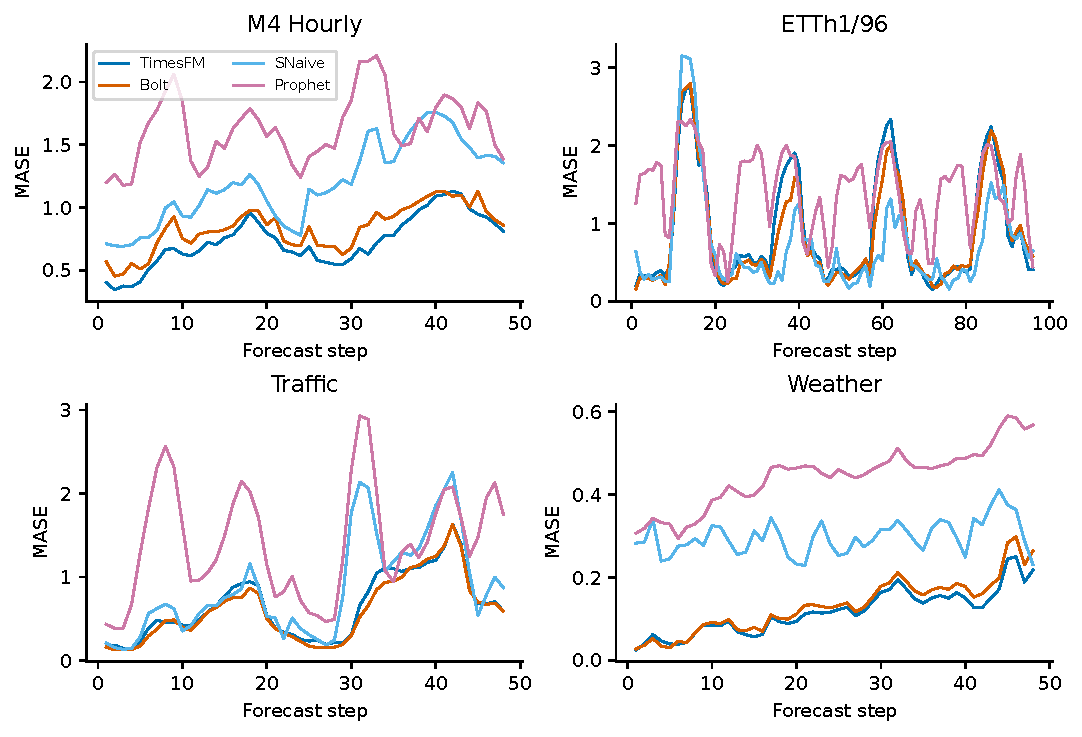
\includegraphics[width=\linewidth]{img/experiments/horizon_mase.pdf}
\caption{MASE at each forecast step for the same tasks and models as Figure~\ref{fig:horizons}. Denominators use the full training series.}\label{fig:horizonmase}
\end{figure}
\begin{table}[!htbp]
\centering
\caption{All saved context-study scores ($\downarrow$); no validation selection.}
\label{tab:contexts}
\small
\setlength{\tabcolsep}{3.5pt}
\begin{tabular}{lrrr}
\hline
Task & Context & sMAPE & MASE \\
\hline
M4 Hourly & 512 & 8.664 & 0.7337 \\
M4 Hourly & 1024 & 8.606 & 0.7336 \\
M4 Hourly & 2048 & 8.606 & 0.7336 \\
M4 Hourly & 4096 & 8.606 & 0.7336 \\
M4 Hourly & 8192 & 8.606 & 0.7336 \\
M4 Hourly & 16256 & 8.606 & 0.7336 \\
ETTh1/48 & 512 & 37.274 & 0.7051 \\
ETTh1/48 & 1024 & 32.961 & 0.5677 \\
ETTh1/48 & 2048 & 31.569 & 0.5430 \\
ETTh1/48 & 4096 & 34.719 & 0.6072 \\
ETTh1/48 & 8192 & 34.672 & 0.6332 \\
ETTh1/48 & 16256 & 33.920 & 0.6181 \\
ETTm1/48 & 512 & 35.345 & 0.4545 \\
ETTm1/48 & 1024 & 35.690 & 0.4571 \\
ETTm1/48 & 2048 & 38.246 & 0.5143 \\
ETTm1/48 & 4096 & 35.718 & 0.4308 \\
ETTm1/48 & 8192 & 36.277 & 0.4426 \\
ETTm1/48 & 16256 & 36.086 & 0.4668 \\
Weather & 512 & 44.872 & 0.1327 \\
Weather & 1024 & 39.880 & 0.1176 \\
Weather & 2048 & 45.276 & 0.1225 \\
Weather & 4096 & 37.882 & 0.1148 \\
Weather & 8192 & 33.724 & 0.1329 \\
Weather & 16256 & 42.058 & 0.1369 \\
\hline
\end{tabular}
\end{table}

